\documentclass[
    12pt,
    a4paper,
    ngerman,
    color=3b,% Farbe für Hervorhebungen auf Basis der Deklarationen in den
    %type=intern,
    %titlepage=true,
    marginpar=false,
    colorback=false,
    %logo=head,
    leqno,
]{tudaexercise}
\usepackage{import}
% Import all Packages from Main Preamble with relative Path
\subimport*{../../}{preamble}
% Get Labels from Main Document using the xr-hyper Package
\externaldocument{../../AuD-Zusammenfassung-2020}
% Set Graphics Path, so pictures load correctly
\graphicspath{{../../}}

\begin{document}
\section{Graph Algorithms}\index{Graph Algorithms}
\subsection{Graphen}\index{Graphen}
    \begin{itemize}
        \item \fatsf{(Endlicher) gerichteter Graph}
            \begin{itemize}
                \item (endlicher) gerichteter Graph $G = (V,E)$
                \item besteht aus (endlicher) Knotenmenge $V$
                \item besteht aus (endlicher) Kantenmenge $E \subseteq V x V$
                \item $(u,v) \in E$: Kanten von Knoten $u$ zu $v$
                \item Kanten haben eine Richtung
            \end{itemize}

        \item \fatsf{Ungerichtete Graphen}
            \begin{itemize}
                \item (endlicher) ungerichteter Graph $G = (V,E)$
                \item besteht aus (endlicher) Knotenmenge $V$
                \item besteht aus (endlicher) Kantenmenge $E \subseteq V x V$, sodass $(u,v) \in E \Leftrightarrow (v,u) \in E$
                \item Kanten haben keine Richtung
            \end{itemize}

        \item \fatsf{Pfadfinder}\index{Pfadfinder}
            \begin{itemize}
                \item Knoten $v$ ist von Knoten $u$ erreichbar, wenn es einen Pfad gibt
                \item $u$ ist immer von $u$ per leerem Pfad (k=1) erreichbar
                \item Länge des Pfades = $k - 1$ = Anzahl Kanten
            \end{itemize}

        \item \fatsf{Zusammenhänge}\index{Zusammenhänge}
            \begin{itemize}
                \item Ungerichtet: Zusammenhängend\index{Zusammenhänge!zusammenhängend} wenn jeder Knoten von jedem anderen Knoten aus erreichbar ist
                \item Gerichtet: \fatsf{Stark}\index{Zusammenhänge!stark zusammenhängend} zusammenhängend, wenn obiges auch gemäß Kantenrichtung gilt
            \end{itemize}

        \item \fatsf{Bäume und Subgraphen} \\
            Graph $G$ ist ein Baum, wenn $V$ leer ist oder wenn es einen Knoten in $V$ gibt, \\
            von dem aus jeder andere Knoten eindeutig erreichbar ist (Wurzel). \\
            Graph $G'=(V',E')$ ist Subgraph\index{Subgraph} von $G=(V,E)$, wenn $V'\subseteq V$ und $E' \subseteq E$.

        \item \fatsf{Darstellung von Graphen}
            \begin{itemize}
                \item Als Adjazentmatrix\index{Adjazenzmatrix} (1, wenn Kante von i zu j / 0, wenn keine Kante)
                \item Bei ungerichteten Graphen ist Matrix spiegelsymmetrisch zur Hauptdiagonalen
                \item Speicherbedarf: $\Theta(|V^2|)$
                \item[]
                    \begin{minipage}{0.45\textwidth}
                        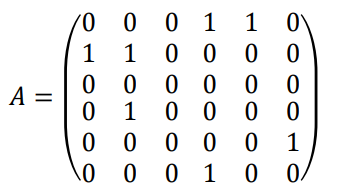
\includegraphics[width=4cm]{pictures/graph1.PNG}
                    \end{minipage}
                    \begin{minipage}{0.45\textwidth}
                        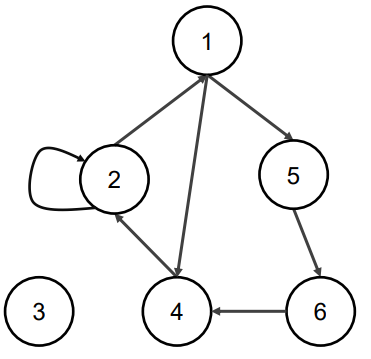
\includegraphics[width=4cm]{pictures/graph2.PNG}
                    \end{minipage}
                \item Auch darstellbar als Array mit verketteten Listen
                \item Speicherbedarf: $\Theta(|V| + |E|)$
            \end{itemize}

        \item \fatsf{Gewichtete Graphen}\index{Gewichtete Graphen}
            \begin{itemize}
                \item gewichteter gerichteter Graph $G=(V,E)$
                \item besitzt zusätzlich Funktion $w: E \rightarrow R$
                \item Abspeichern des Werts einer Kante $w((u,v))$
            \end{itemize}
    \end{itemize}

\subsection{Breadth-First Search (BFS)}\index{Breadth-First Search (BFS)}
    \begin{itemize}
        \item \fatsf{Idee}
            \begin{itemize}
                \item Besuche zuerst alle unmittelbaren Nachbarn, dann deren Nachbarn, usw.
                \item Anwendung: Webcrawling, Garbage Collection,..
            \end{itemize}
        
        \item \fatsf{Algorithmus}
            \begin{itemize}
                \item[]
                    \begin{ccode}[autogobble,escapeinside=||]{title={BFS(G,s) //G=(V,E) s = source node in V}}
                        BFS(G,s) //G=(V,E) s = source node in V

                        FOREACH u in V-{s} DO
                            u.color = WHITE;        // Weiß = noch nicht besucht
                            u.dist = |$+\infty$|            // Setzen der Distanzen auf Unendlich
                            u.pred = nil;           // Setzen der Vorgänger auf nil
                        s.color = GRAY;             // Anfang bei Startnode
                        s.dist = 0;
                        s.pred = nil;
                        newQueue(Q);
                        enqueue(Q,s);
                        WHILE !isEmpty(Q) DO
                            u = dequeue(Q); 
                            FOREACH v in adj(G,u) DO
                                IF v.color == WHITE THEN
                                    v.color == GRAY;
                                    v.dist = u.dist+1;
                                    v.pred = u;
                                    enqueue(Q,v);
                            u.color = BLACK;            // Knoten abgearbeitet
                    \end{ccode}
                \item[] \begin{tcolorbox}[
                    colback=yellow!20,
                    colframe=black!50!red!100,
                    enhanced,
                    title={Farben:}
                ]
                \begin{itemize}
                    \item {\makebox[\widthof{\texttt{WHITE}:}][l]{\texttt{WHITE}:} Knoten noch nicht besucht}
                    \item {\makebox[\widthof{\texttt{WHITE}:}][l]{\texttt{GRAY}:} Knoten in Queue für nächsten Schritt}
                    \item {\makebox[\widthof{\texttt{WHITE}:}][l]{\texttt{BLACK}:} Knoten ist Fertig}
                \end{itemize}
                \end{tcolorbox}
                \item Laufzeit: $O(|V| + |E|)$
                \item Nach Algorithmus steht in $v$ die kürzeste Distanz von $s$ nach $v$
            \end{itemize}

\pagebreak

        \item \fatsf{Kürzeste Pfade ausgeben}
            \begin{itemize}
                \item[]
                    \begin{ccode}[autogobble]{title={print-path(G,s,v) // Assumes that BFS(G,s) has already been executed}}
                    IF v == s THEN
                        print s;
                    ELSE
                        IF v.pred == nil THEN
                            print "no path from s to v"
                        ELSE
                            print-path(G,s,v.pred);
                            print v;
                    \end{ccode}
            \end{itemize}

        \item \fatsf{Abgeleiteter BFS-Baum}
            \begin{itemize}
                \item[] 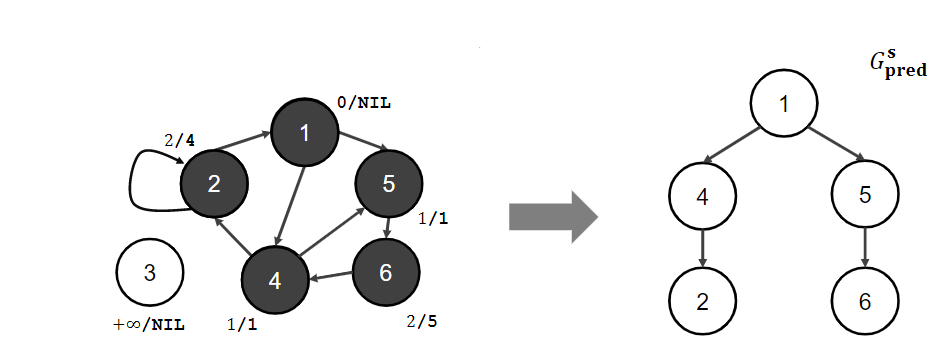
\includegraphics[width=14cm]{pictures/bfsBaum.PNG}
                \item Subgraph $G^s_{pred} = (V^s_{pred},E^s_{pred})$ von G:
                    \begin{itemize}
                        \item $V^s_{pred} = \{v \in V | v.pred \neq nil\} \cup \{s\}$
                        \item $E^s_{pred} = \{(v.pred,v) | v \in V^s_{pred} - \{s\}\}$
                    \end{itemize}
                \item $G^s_{pred}$ enthält alle von $s$ aus erreichbaren Knoten in $G$
                \item Außerdem handelt es sich hier nur um kürzeste Pfade
            \end{itemize}
    \end{itemize}

\subsection{Depth-First Search(DFS)}\index{Depth-First Search(DFS)}
    \begin{itemize}
        \item \fatsf{Idee}
            \begin{itemize}
                \item Besuche zuerst alle noch nicht besuchten Nachfolgeknoten
                \item \string"Laufe so weit wie möglich weg vom aktuellen Knoten\string"
            \end{itemize}

        \item \fatsf{Algorithmus}
            \begin{itemize}
                \item[]
                    \begin{ccode}[autogobble]{title={ DFS(G)}}
                    FOREACH u in V DO
                        u.color = WHITE;
                        u.pred = nil;
                    time = 0;               // time hier als globale Variable
                    FOREACH u in v DO
                        IF u.color == WHITE THEN
                            DFS-VISIT(G,u)  // Start eines rekursiven Aufrufs
                    \end{ccode}
                \item[]
                    \begin{ccode}[autogobble]{title={DFS-VISIT(G,u)}}
                    time = time + 1;
                    u.disc = time;          // discovery time
                    u.color = GRAY;
                    FOREACH v in adj(G,u) DO
                        IF v.color == WHITE THEN
                            v.pred = u;
                            DFS-VISIT(G,v);
                    u.color = BLACK;
                    time = time + 1;
                    u.finish = time;        // finish time
                    \end{ccode}
            \end{itemize}

        \item \fatsf{DFS-Wald = Menge von DFS-Bäumen}\index{DFS-Wald}
            \begin{itemize}
                \item Subgraph $G_{pred}=(V,E_{pred})$ von G
                \item besteht aus $E_{pred} = {(v.pred,v)|v \in V, v.pred \neq nil}$
                \item DFS-Baum gibt nicht unbedingt den kürzesten Weg wieder
                \item[] 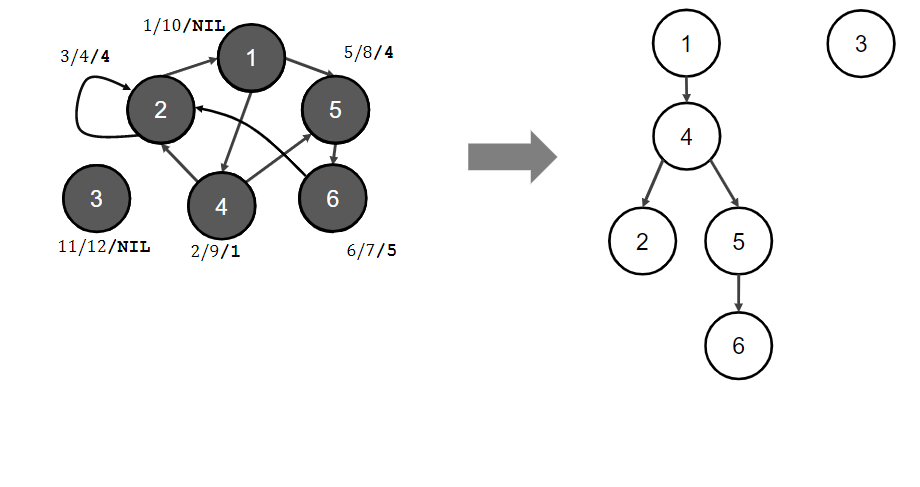
\includegraphics[width=9cm]{pictures/dfswald.PNG}
            \end{itemize}
        \vspace*{-2cm}
        \item \fatsf{Kantenarten}
            \begin{itemize}
                \item {\makebox[3cm][l]{Baumkanten:}} alle Kanten in $G_{pred}$
                \item {\makebox[3cm][l]{Vorwärtskanten:}} alle Kanten in $G$ zu Nachkommen in $G_{pred}$, die nicht Baumkante
                \item {\makebox[3cm][l]{Rückwärtskanten:}} alle Kanten in $G$ zu Vorfahren in $G_{pred}$, die nicht Baumkante
                \item {\makebox[3cm][l]{Kreuzkanten:}} alle anderen Kanten in $G$ (inkl. Schleifen)
            \end{itemize}

        \item \fatsf{Anwendungen DFS}
            \begin{itemize}
                \item Job Scheduling (Job X muss vor Job Y beendet sein)
                \item Topologisches Sortieren
                    \begin{itemize}
                        \item nur für dag (directed acyclic graph)
                        \item Kanten immer nur nach rechts
                        \item Sortierung aber nicht eindeutig
                        \item[] 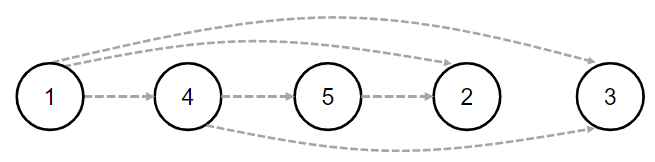
\includegraphics[width=8cm]{pictures/topo.PNG}
                        \item[]
                            \begin{ccode}[autogobble]{title={TOPOLOGICAL-SORT(G)}}
                            new LinkedList(L);
                            run DFS(G) but, each time a node is finished, insert in front of L
                            return L.head;
                            \end{ccode} 
                    \end{itemize}
            \end{itemize}
        
\pagebreak

        \item \fatsf{Starke Zusammenhangskomponenten}\index{Starke Zusammenhangskomponenten}
            \begin{itemize}
                \item Knotenmenge $C \subseteq V$, so dass
                \item[] es zwischen zwei Knoten $u,v \in C$ einen Pfad von $u$ nach $v$ gibt
                \item[] und es keine Menge $D \subseteq V$ mit $C \subsetneq D$ gibt, für die obiges auch gilt.
                \item[] 
                \item[]
                    \begin{minipage}{0.35\textwidth}
                        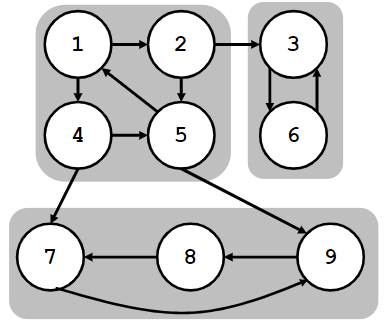
\includegraphics[width=6cm]{pictures/scc.PNG}
                    \end{minipage} 
                    \begin{minipage}{0.55\textwidth}
                    Eigenschaften:
                        \begin{itemize}
                            \item Verschiedene SCC's sind disjunkt
                            \item Zwei SCC's sind nur in eine Richtung verbunden
                        \end{itemize}
                    \end{minipage}
                \item Algorithmus:
                    \begin{itemize}
                        \item DFS zweimal laufen lassen
                        \item[] Einmal auf Graph $G$
                        \item[] Einmal auf Graph $G^T = (V,E^T)$ (transponiert)
                        \item Dadurch bleiben die SCC's gleich, die Kanten drehen sich aber jeweils um
                        \item Code:
                        \item[]
                            \begin{ccode}[autogobble,escapeinside=||]{title={SCC(G)}}
                            run DFS(G)
                            compute |$G^T$|
                            run DGS(|$G^T$|) but visit vertices in main loop
                                in descending finish time from 1
                            output each DFS tree from above as one SCC
                            \end{ccode}
                    \end{itemize}
            \end{itemize}
    \end{itemize}
\clearpage
\subsection{Minimale Spannbäume}\index{Minimale Spannbäume}
    \begin{itemize}
        \item \fatsf{Definition}
            \begin{itemize}
                \item Verbindung aller Knoten miteinander
                \item Minimaler Spannbaum $\Rightarrow$ Minimales Gewicht
            \end{itemize}

        \item \fatsf{Allgemeiner Algorithmus}
            \begin{itemize}
                \item[]
                    \begin{ccode}[autogobble,escapeinside=||]{title={genericMST(G,w)}}
                    A = |$\emptyset$|
                    WHILE A does not form a spanning tree for G DO
                        find safe edge {u,v} for A
                        A = A |$\cup$|{{u,v}}
                    return A
                    \end{ccode}
                \item[]
                    \begin{minipage}{0.35\textwidth}
                        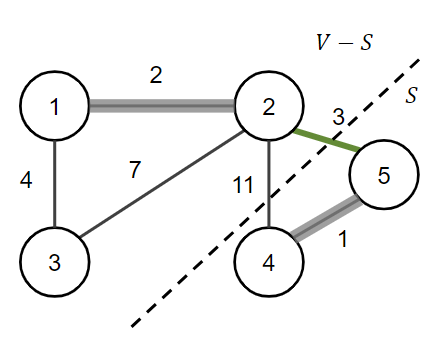
\includegraphics[width=6cm]{pictures/mstTerm.PNG}
                    \end{minipage}
                    \begin{minipage}{0.55\textwidth}
                        Terminologie:
                            \begin{itemize}
                                \item Schnitt (S, V-S) partioniert Knoten in zwei Mengen
                                \item \{u,v\} überbrückt Schnitt, wenn $u \in S$ und $v \in V-S$
                                \item Schnitt respektiert $A \subseteq E$, wenn keine Kante \{u,v\} aus A den Schnitt überbrückt
                                \item \{u,v\} leichte Kante für (S, V-S), wenn w(\{u,v\}) minimal für alle den Schnitt überbrückenden Kanten
                                \item \{u,v\} sicher für A, wenn $A \cup \{\{u,v\}\}$ Teilmenge eines MST
                            \end{itemize}
                    \end{minipage}
            \end{itemize}
        
        \item \fatsf{Algorithmus von Kruskal}\index{Kruksal}
            \begin{itemize}
                \item Lässt parallel mehrere Unterbäume eines MST wachsen
                \item In Worten: Suchen der \string"kleinsten\string" Kante und Zusammenfügen von Mengen, falls noch nicht geschehen
                \item Laufzeit: $O(|E| \cdot log|E|)$
                \item[]
                    \begin{ccode}[autogobble,escapeinside=||,fontsize=\small]{title={MST-Kruskal(G,w)}}
                    A = |$\emptyset$|
                    FOREACH v in V DO
                        set(v) = {v};       // Menge mit sich selbst
                    Sort edges according to weight in nondecreasing order
                    FOREACH {u,v} in E according to order DO
                        IF set(u) != set(v) THEN    // Mengen noch nicht verbunden
                            A = A |$\cup$| {{u,v}}; 
                            UNION(G,u,v);   // Zusammenführen der Mengen aller Knoten aus den Sets
                    return A;
                    \end{ccode}
            \end{itemize}
            \clearpage
        \item \fatsf{Algorithmus von Prim}\index{Prim}
            \begin{itemize}
                \item Konstruiert einen MST Knoten für Knoten
                \item Fügt immer leichte Kante zu zusammenhängender Menge hinzu
                \item Laufzeit: $O(|E| + |V| \cdot log|V|)$
                \item[]
                    \begin{ccode}[autogobble,escapeinside=||]{title={MST-Prim(G,w,r) // r is given root}}
                    FOREACH v in V DO 
                        v.key = +|$\infty$|;
                        v.pred = nil;
                    r.key = -|$\infty$|
                    Q = V;
                    WHILE !isEmpty(Q) DO
                        u = EXTRACT-MIN(Q);     // smallest key value
                        FOREACH v in adj(u) DO
                            IF v|$\in$|Q and w({u,v})<v.key THEN
                                v.key = w({u,v});
                                v.pred = u;
                    \end{ccode}
            \end{itemize}
        
    \end{itemize}

\subsection{Kürzeste Wege in (gerichteten) Graphen}\index{Kürzeste Wege}
    \begin{itemize}
        \item \fatsf{Definition}
            \begin{itemize}
                \item SSSP - Single-Source Shortest Path\index{SSSP}
                \item Von Quelle $s$ ausgehend die kürzesten Pfad zu allen anderen Knoten
                \item Kürzester Pfad: Minimales Gewicht von einem zum anderen Knoten
                \item BFS findet nur minimale Kantenwege (nicht Gewichtswege)
                \item MST minimiert das Gesamtgewicht des Baumes (nicht zu einzelnen Kanten)
                \item Negative Kantengewichte sind erlaubt, aber keine Zyklen mit negativem Gesamtgewicht
            \end{itemize}
        
        \item \fatsf{Gemeinsame Idee für Algorithmen - Relax}\index{Relax}
            \begin{itemize}
                \item Verringere aktuelle Distanz von Knoten $v$, wenn durch Kante $(u,v)$ kürzer erreichbar
                \item[] 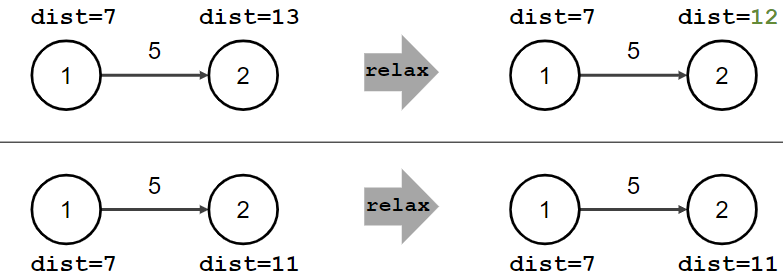
\includegraphics[width=12cm]{pictures/ssspRelax.PNG}
                \item[]
                    \begin{ccode}[autogobble]{title={relax(G,u,v,w)}}
                    IF v.dist > u.dist + w((u,v)) THEN
                        v.dist = u.dist + w((u,v));
                        v.pred = u;
                    \end{ccode}
            \end{itemize}
\clearpage
        \item \fatsf{Bellman-Ford-Algorithmus}\index{Bellman-Ford}
            \begin{itemize}
                \item Laufzeit: $\Theta(|E| \cdot |V|)$
                \item[]
                    \begin{ccode}[autogobble,escapeinside=||]{title={Bellman-Ford-SSSP(G,s,w)}}
                    initSSSP(G,s,w);
                    FOR i = 1 TO |$\vert V\vert$|-1 DO
                        FOREACH (u,v) in E DO
                            relax(G,u,v,w);
                    FOREACH (u,v) in E DO   // Prüfung ob negativer Zyklus
                        IF v.dist > u.dist+w((u,v)) THEN
                            return false;
                    return true;
                    \end{ccode}
                    \begin{ccode}[autogobble,escapeinside=||]{title={initSSSP(G,s,w)}}
                    FOREACH v in V DO
                        v.dist = |$\infty$|;
                        v.pred = nil;
                    s.dist = 0;
                    \end{ccode}
            \end{itemize}

        \item \fatsf{TopoSort für dag}\index{TopoSort}
            \begin{itemize}
                \item Erhalten des kürzesten Pfades durch das topologische Sortieren
                \item Laufzeit: $\Theta(|E| + |V|)$
                \item[]
                    \begin{ccode}[autogobble]{title={TopoSort-SSSP(G,s,w)    // G muss dag sein}}
                    initSSSP(G,s,w);
                    execute topological sorting
                    FOREACH u in V in topological order DO
                        FOREACH v in adj(u) DO
                            relax(G,u,v,w);
                    \end{ccode}
            \end{itemize}

        \item \fatsf{Dijkstra-Algorithmus}\index{Dijkstra}
            \begin{itemize}
                \item Voraussetzung: Keine negativen Kantengewichte
                \item Laufzeit: $\Theta(|V| \cdot log|V| + |E|)$
                \item[]
                    \begin{ccode}[autogobble]{title={Dijkstra-SSSP(G,s,w)}}
                    initSSSP(G,s,w);
                    Q = V;
                    WHILE !isEmpty(Q) DO
                        u = EXTRACT-MIN(Q);     // smallest distance
                        FOREACH v in adj(u) DO
                            relax(G,u,v,w);
                    \end{ccode}
                \item \begin{minipage}{.3\textwidth}
                    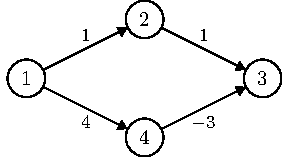
\includegraphics[]{pictures/dijkstra-fail-graph/dijkstra-fail-graph}
                \end{minipage}
                \begin{minipage}{.5\textwidth}
                    \begin{itemize}
                        \item Beispiel für Problem mit negativen Kantengewisten bei Dijkstra: Dijkstra würde Pfad 1-2-3 liefern, da das Kantengewicht 4 größer als der andere Pfad ist.
                    \end{itemize}
                \end{minipage}
            \end{itemize}
    \end{itemize}
\clearpage
\subsection{Maximaler Fluss in Graphen}\index{Maximaler Fluss}
    \begin{itemize}
        \item \fatsf{Idee}
            \begin{itemize}
                \item[]
                    \begin{minipage}{0.35\textwidth}
                        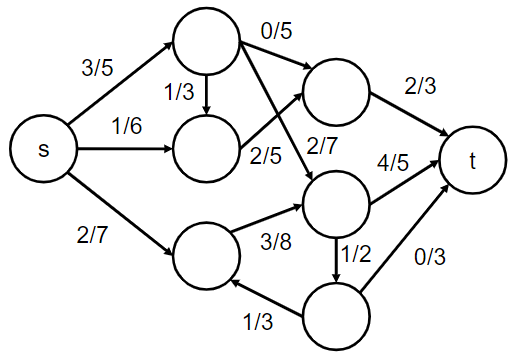
\includegraphics[width=7cm]{pictures/flussIdee.PNG}
                    \end{minipage}
                    \begin{minipage}{0.55\textwidth}
                        \begin{itemize}
                            \item Kanten haben Flusswert und maximale Kapazität
                            \item Jeder Knoten (außer s und t) haben den gleichen eingehenden und ausgehenden Fluss
                            \item Ziel: Finde maximalen Fluss von s nach t
                            \item s: Source/Quelle
                            \item t: Target/Senke
                        \end{itemize}
                    \end{minipage}
                \item \fatsf{Flussnetzwerk:} \\
                        Ein Flussnetzwerk\index{Flussnetzwerk} ist ein gewichteter, gerichteter Graph $G=(V,E)$ mit Kapazität $c$, so dass
                        $c(u,v) \geq 0$ für $(u,v) \in E$ und $c(u,v) = 0$ für $(u,v) \notin E$, mit zwei Knoten $s,t \in V$,
                        so dass jeder Knoten von $s$ aus erreichbar ist und $t$ von jedem Knoten aus erreichbar ist. 
                        Damit gilt $|E| \geq |V| - 1$.
                \item \fatsf{Fluss:}\index{Fluss} \\
                        Ein Fluss $f: V x V \rightarrow \mathbb{R}$ für ein Flussnetzwerk $G = (V,E)$ mit Kapazität $c$
                        und Quelle $s$ und Senke $t$ erfüllt $0 \leq f(u,v) \leq c(u,v)$ für alle $u,v \in V$, sowie für alle
                        $u \in V - \{s,t\}$: \\ 
                        $\sum_{v\in V} f(u,v) = \sum_{v\in V} f(v,u)$ (ausgehend = eingehend)
                \item \fatsf{Wert eines Flusses} \\
                        Der Wert $|f|$ eines Flusses $f: V x V \rightarrow \mathbb{R}$ für ein Flussnetzwerk $G$ ist: \\
                        $|f| = \sum_{v\in V} f(s,v) = \sum_{v\in V} f(v,s)$
            \end{itemize}

        \item \fatsf{Transformationen}
            \begin{itemize}
                \item[] 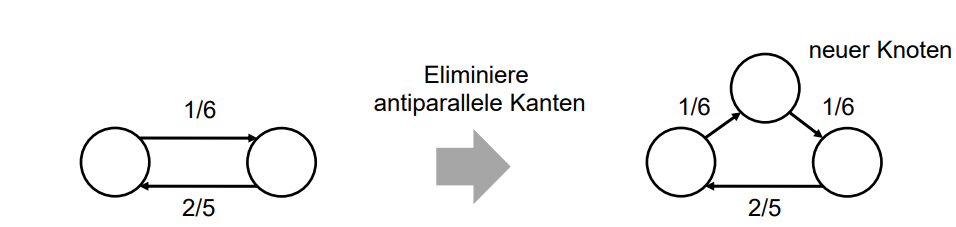
\includegraphics[width=12cm]{pictures/flussTrans1.PNG}
                \item[] 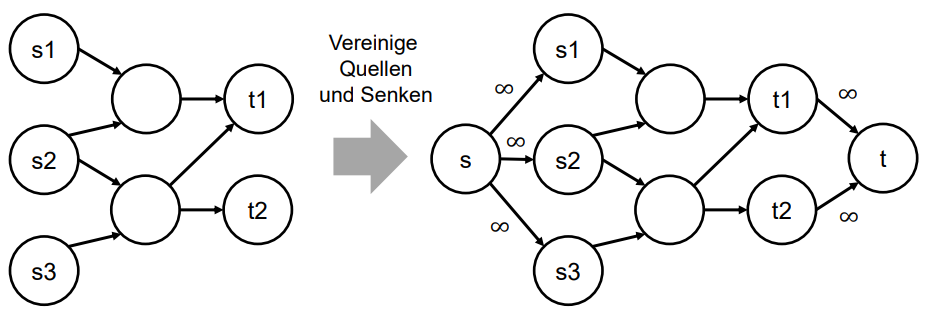
\includegraphics[width=12cm]{pictures/flussTrans2.PNG}
            \end{itemize}
\clearpage
        \item \fatsf{Restkapazitätsgraph}\index{Restkapazitätsgraph}
            \begin{itemize}
                \item Wird für Ford-Fulkerson benötigt
                \item Restkapazität $c_f(u,v)$: \\
                        \centerline{$c_f(u,v) = \begin{cases}
                                                c(u,v) - f(u,v) & \text{falls $(u,v) \in E$} \\
                                                f(v,u) & \text{falls $(v,u) \in E$} \\
                                                0 & \text{sonst}
                                                \end{cases}$}
                \item $G_f = (V, E_f)$ mit $E_f = \{(u,v) \in V x V | c_f(u,v) > 0 \}$
                \item[] \includegraphics[width=12cm]{pictures/restkapazitätsgraph.PNG}
                \item Suche eines Pfades von $s$ nach $t$ und Erhöhung aller Flüsse um niedrigsten möglichen Wert auf Pfad
            \end{itemize}


        \item \fatsf{Ford-Fulkerson-Algorithmus}\index{Ford-Fulkerson}
            \begin{itemize}
                \item Idee: Suche Pfad von $s$ nach $t$, der noch \fatsf{erweiterbar} ist
                \item Suche dieses Pfades im Restkapazitätsgraphen $G_f$ (mögliche Zu- und Abflüsse)
                \item Code:
                \item[]
                    \begin{ccode}[autogobble,escapeinside=||]{title={Ford-Fulkerson(G,s,t,c)}}
                    FOREACH e in E do e.flow = 0;
                    WHILE there is path p from s to t in |$G_{flow}$| DO
                        |$c_{flow}(p)$| = min {|$c_{flow}(u,v)$| : (u,v) in p}
                        FOREACH e in p DO
                            IF e in E THEN
                                e.flow = e.flow + |$c_{flow}(p)$|;
                            ELSE
                                e.flow = e.flow - |$c_{flow}(p)$|;
                    \end{ccode}
                \item Die Pfadsuche erfolgt z.B. per BFS oder DFS
                \item Laufzeit: $O(|E| \cdot u \cdot |f^*|)$ \\
                        ($O(|V| \cdot |E|^2)$ Mit Verbesserung nach Edmonds-Karp) \\
                        (wobei $f^*$ maximaler Fluss und Fluss um bis zu $\frac{1}{u}$ pro Iteration wächst)
\pagebreak
                \item Beispiel:
                \item[] 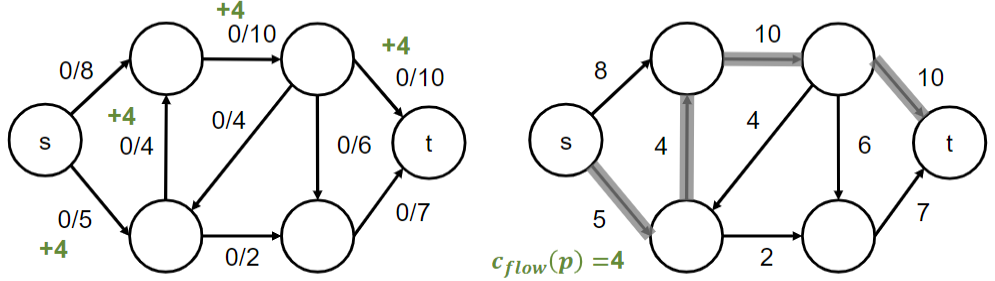
\includegraphics[width=12cm]{pictures/fordbsp1.PNG}
                \item[] 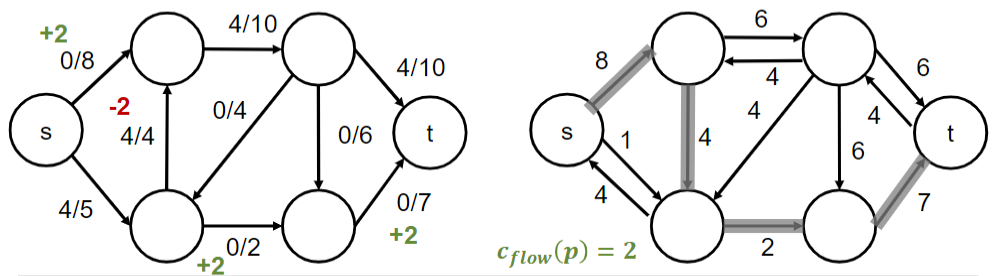
\includegraphics[width=12cm]{pictures/fordbsp2.PNG}
            \end{itemize}
    \end{itemize}
\clearpage
\end{document}
